This chapter describes how the simulation model of the experimental data center POD 2 at \gls{rsn} was constructed using the \gls{lua}-to-\gls{cuda} code generation \gls{api} built into RAFSINE.

The server racks in the data center were configured in a so called hot aisle configuration, so that the backside of each row of server racks were facing one another. As hot air gathered in the aisle, it pooled along the ceiling, after which it was drawn into the inlets of four \gls{crac} along the sides of the room. The \gls{crac}s were configured to cool the air from inlets on top of them using heat exchange elements, and then blow the cold air out into the room. Figure~\ref{fig:flow} illustrates this setup.

%\begin{figure}[!htb]
%\begin{center}
%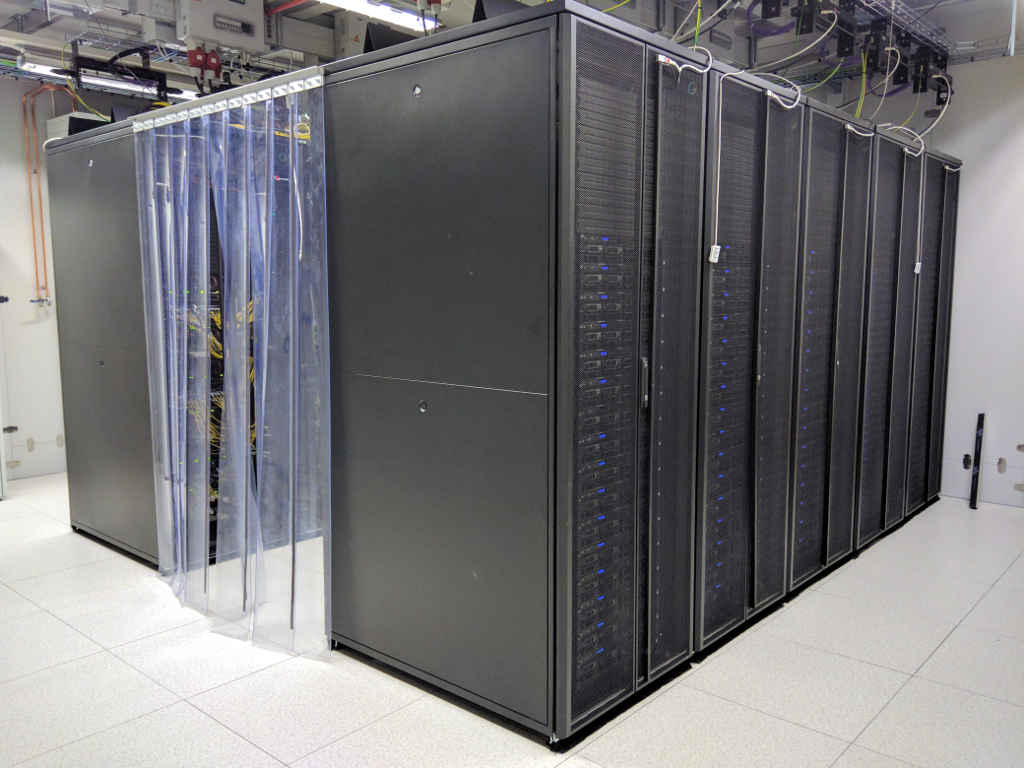
\includegraphics[width=0.65\linewidth]{pod2_interior.jpg}
%\end{center}
%\caption{The interior of data center module POD 2 at \gls{rsn}.}
%\end{figure}

\begin{figure}[!htb]
\centering
\begin{small} % For text embedded in figure
\def\svgwidth{0.65\linewidth}
\input{Figures/flow.pdf_tex}
\end{small}
\caption{Theoretical heat flow in the data center POD 2 at \gls{rsn}.}
\label{fig:flow}
\end{figure}

\begin{figure}[!htb]
\centering
\begin{scriptsize} % For text embedded in figure
\def\svgwidth{\linewidth}
\input{Figures/pod2_schematic.pdf_tex}
\end{scriptsize}
\caption{Schematic of the data center module POD 2 at \gls{rsn}.}
\label{fig:floor_plan}
\end{figure}

\clearpage

\section{Data Center CFD Model} \label{sec:modeling}
The basic geometry of the boundary conditions in RAFSINE were defined in a \gls{lua} script file, based on length measurements of the physical data center, as seen in figure~\ref{fig:floor_plan}. \gls{lbm} is based on a discreet lattice of cells, and the program automatically discretized the lengths from meters into lattice units ($lu$).

For simplicity, the model used the same lattice types as the example simulation model included in the original RAFSINE code, which was D3Q19 for the velocity distribution functions and D3Q6 for the temperature.

Since the domain of \gls{lbm} is based on a regular grid with Euclidian coordinates for each cell, modeling sloped surfaces is problematic unless a very high resolution is used. Figure~\ref{fig:crac} shows an approximation of how the \gls{crac}s were modeled. As can be seen, the geometry was simplified to remove slopes, while the areas of the topside inlet and sideways exhaust kept the same dimensions.

The floor, walls and ceiling of the room were modeled using the half-way bounce-back scheme explained in chapter~\ref{sec:boundary_step}, which basically defines zero air velocity along these boundaries. Likewise, the temperature distribution functions were also implemented with bounce-back which meant no heat transfer took place at the walls. The boundary conditions for the \gls{crac}s and servers required more specialized definitions.

\begin{figure}[!htb]
\centering
\begin{scriptsize} % For text embedded in figure
\def\svgwidth{0.5\linewidth}
\input{Figures/cooler.pdf_tex}
\end{scriptsize}
\caption{Heat exchange cooler SEE Cooler HDZ-2.}
\label{fig:crac}
\end{figure}
\clearpage
\subsubsection{CRACs}
Firstly, the air exhausts at the sides of the \gls{crac}s were set to blow cold air at a constant temperature $T_{supply}$ and flow rate $Q_{supply}$. Secondly, the topside inlets were set to create a constant static pressure $p_{return}$, which meant setting the gradient of the velocity and temperature fields to zero, that is~\cites[pg.164]{Delbosc}
\begin{equation}
\frac{\partial\vec{u}}{\partial z}=0,~\frac{\partial T}{\partial z}=0.
\end{equation}
This von Neumann boundary condition  is called \textit{zero-gradient}. $\partial z$ is the gradient component corresponding to the normal of the inlet plane. Since these two boundary conditions modeled a circulating air flow, the inlet flow rate $Q_{return} = Q_{supply}$.

\begin{figure}[!htb]
\centering
\begin{scriptsize} % For text embedded in figure
\def\svgwidth{\linewidth}
\input{Figures/racks.pdf_tex}
\end{scriptsize}
\caption{Two rows of five Minkels server racks positioned in hot aisle configuration. The entrance is separated by a curtain of flexible plastic sheets.}
\label{fig:racks}
\end{figure}

\subsubsection{Server racks}
Although in reality, each server rack contained between 16-30 servers, their power consumption was only measured on a per-rack basis. Since their individual power usages were unknown specific boundary conditions for each server could not be derived. Instead each rack was modeled using one inlet boundary condition on the front of the rack and one exhaust on the back. Figure~\ref{fig:racks} illustrates the modeling of the racks.

The air inlet on the front of the racks were modeled using a similar zero-gradient boundary condition as the \gls{crac} inlets, with a constant flow rate $Q_{in}$.

Each server contained case mounted fans which provided cooling to the components depending on their temperatures. When the server components consumed more power and created more heat, the fans automatically increased their flow rates $Q_{out}$. The temperatures on the back of the server racks $T_{out}$ was therefore based on the temperatures on the front $T_{in}$ plus a temperature increase $\Delta T$ which depended on server power consumption. This created the relations~\cites[pg.166]{Delbosc}
\begin{align}
T_{out} &= \frac{\int T_{in} dA}{\int dA} + \Delta T,\\
\vec{u}_{out} &= \frac{Q_{out}}{\int dA} \vec{n},
\end{align}
which describes the boundary condition for the temperature and velocity distribution functions on the back of the racks. The first equation is the average of the integration of inlet air $T_{in}$ over an area $A$, which in this case was simply the six temperature distribution functions of an inlet lattice cell in the D3Q6 model. The second shows the exhaust air velocity along the normal $\vec{n}$ of each cell on the server backside.

Temperature increase $\Delta T$ is affected by the server workload, which relates directly to its power consumption $P$ (measured in kilowatts) and fan flow rate $Q_{out}$. This was modeled using the relation~\cites[pg.167]{Delbosc}
\begin{equation}
\Delta T = \frac{P \cdot \nu}{Q_{out} \cdot k \cdot Pr},
\end{equation}
where the constants $\nu = 1.568\cdot10^{-5}$ m$^2$/s is the kinematic viscosity, $k=2.624\cdot10^{-5}$ kW/m is the thermal conductivity and $Pr = 0.707$ is the Prandtl number of air at 30\degree C\footnote{The Engineering ToolBox: Dry Air Properties \url{https://www.engineeringtoolbox.com/dry-air-properties-d_973.html} }.

Figure \ref{fig:pod2_voxel} shows a screenshot of the geometry of the final data center model as implemented in RAFSINE. The ceiling was removed for better visibility but exists in the actual simulation model.


\section{Simulation Input Data}
As described in chapter~\ref{sec:modeling}, the data center \gls{lbm} model had four unknown input parameters - the volumeteric flow rates and air exhaust temperatures for the four \gls{crac} units, $Q_{supply,i}$ and $T_{supply,i}$ as well as server rack flow rate $Q_{out,j}$ and temperature increase $\Delta T_j$ for $i=1,\dots, 4$ and $j=1,\dots, 10$. Temperature increase depends on rack power consumption $P_j$.

To provide these values, sensor data recorded from an earlier experiment in POD 2 was used, which took place on the 23 of January 2018. The sampling rate of the data was once per minute, and extended a period of 36 hours starting at 9:00.

\clearpage
\subsubsection{CRACs}
The \gls{crac} air flow $Q_{supply}$ rate was measured using a mass flow sensor, which reported flow rate in the unit kg/s. Conversion to m$^3$/s was done using the density of air $\rho=1.177$ kg/m$^3$ at 30\degree C and 1 atm pressure\footnotemark[\value{footnote}]. \gls{crac} air supply temperature $T_{supply}$ was simply measured by a thermometer in \degree C and required no conversion.
\begin{figure}[ht]
\begin{center}
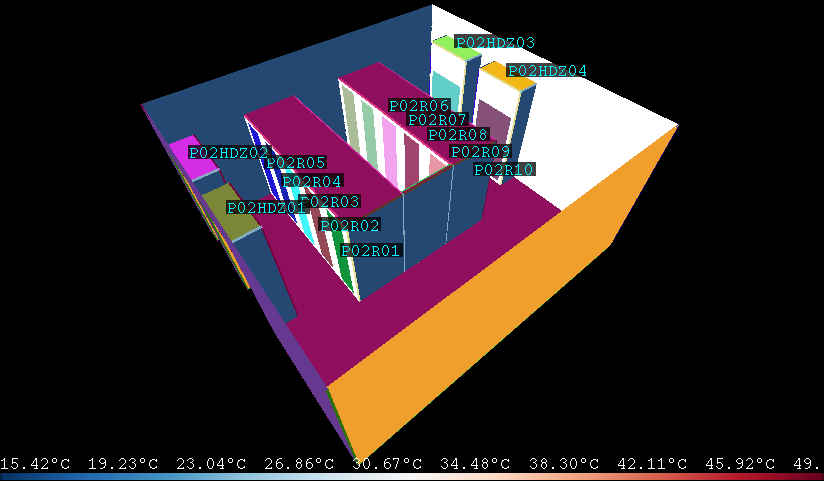
\includegraphics[width=\linewidth]{rafsine_pod2_voxel.jpg}
\end{center}
\caption{Geometry of data center module POD 2.}
\label{fig:pod2_voxel}
\end{figure}

\subsubsection{Server racks}
The server racks were powered by a three-phase power supply, and the recording listed the power consumption of each phase for each rack. The total consumption for each rack $P_j$ was calculated as the sum of the three phases.

Unfortunately, the recording contained no direct measurement of the air flow rate through the server racks, except the rotational speed of the integrated fans measured in rotations per minute (RPM). This meant the flow rate had to be approximated using specifications of the fans inside the racks. Table~\ref{tab:equipment} shows the server equipment installed in each rack, while table~\ref{tab:fans} shows the specifications of the integrated fans.

\begin{table}[h]
\caption{Equipment of the server racks in data center POD 2.}
\begin{center}
    \begin{tabular}{ | l | l | p{1.7cm} |}
    \hline
    \bfseries Rack & \bfseries Equipment & \bfseries Amount $n_{servers}$ \\ \hline
    P02R01 & HPC7000 & 3 \\ \hline
	P02R02 & HPC7000 & 1 \\
	 & Voltaire 4700 & 1 \\ \hline
	P02R03 & HPC7000 & 3 \\ \hline
	P02R04 & Dell R430 & 26 \\ \hline
	P02R05 & Dell R430 & 30 \\ \hline
	P02R06 & Dell R430 & 30 \\ \hline
	P02R07 & Dell R430 & 30 \\ \hline
	P02R08 & Dell R530 & 16 \\ \hline
	P02R09 & Dell R530 & 16 \\ \hline
	P02R10 & Dell R530 & 16 \\ \hline
    \end{tabular}
\end{center}
\label{tab:equipment}
\end{table}

According to the \textit{affinity laws}, the power consumption of a fan is proportional to the cube of the shaft speed. This means the ratio between maximum input power $P_{max}$ and an operational point $P_{op}$ is equal to the cube of ratio maximum fan speed $\omega_{max}$ over operational speed $\omega_{op}$. Around this operating point, the power ratio can be assumed to be proportional to the volumetric flow rates $Q_{max}$ and $Q_{op}$, so
\begin{align}
\frac{P_{max}}{P_{op}} &= \left( \frac{\omega_{max}}{\omega_{op}} \right)^3,\\
\frac{P_{max}}{P_{op}} &= \frac{Q_{max}}{Q_{op}}.
\end{align}
Solving for $Q_{op}$ yields
\begin{equation}
Q_{op} = Q_{max} \left( \frac{\omega_{op}}{\omega_{max}} \right)^{3}.
\end{equation}
As seen in table~\ref{tab:fans}, each Dell R430 and R530 server had $n_{fans}=6$ integrated fans. While the experimental data log recorded the average fan speed of each individual server, this model simplified the boundary conditions for server air flow by using the average fan speed $\omega_{rack}$ in RPM of all servers in a rack. This meant the total flow rate in CFM for a server rack was
\begin{align}
Q_{out} &= \omega_{rack} \cdot n_{fans} \cdot n_{servers} \cdot \frac{Q_{op}}{\omega_{op}}\\
        &= \omega_{rack} \cdot n_{fans} \cdot n_{servers} \cdot Q_{max}\frac{(\omega_{op})^2}{(\omega_{max})^3}.
\end{align}
When calculating air flow for a Dell R430 server at $\approx 50\%$ speed, or 7500 RPM, the total flow $Q_{out}=26$ CFM or 0.0123 m$^3$/s.

A more accurate model would implement a unique boundary condition for each server depending on its own fan speed. Even if the individual power consumption of each server is not recorded, the total consumption of the rack could be divided by the number of servers to get an average for each server.

Because the rotational speeds in racks 1--3 was not recorded, the fan specifications for these servers was not investigated. Instead, the flow rate through these servers was set to scale directly with power usage, by a factor approximated by trial and error.

\begin{table}[h]
\caption{Fan specifications of the servers.}
\begin{center}\small
    \begin{tabular}{ | m{2.2cm} | m{2.9cm} |  m{1.5cm} |  m{2.0cm} |  m{2.2cm} |  m{2.2cm} |}
    \hline
    \bfseries Equipment &  \bfseries Fan type & \bfseries Amount $n_{fans}$ & \bfseries \mbox{Max power} \mbox{$P_{max}$ [W]} & \bfseries \mbox{Max speed} \mbox{$\omega_{max}$ [RPM]} & \bfseries \mbox{Max flow}  \mbox{$Q_{max}$ [CFM]} \\ \hline
	Dell R430 & Delta Electronics GFB0412SHS-DF00 & 6 & 13.2 & 14300 & 30.23 \\ \hline
	Dell R530 & Delta Electronics PFR0612DHE-SP00 & 6 & 19.2 & 14500 & 65.95 \\ \hline
	HP C7000 & Unknown & & & &  \\ \hline
	Voltaire 4700 & Unknown & & & &  \\ \hline
    \end{tabular}
\end{center}
\label{tab:fans}
\end{table}

\section{Simulation Output Data}
The fronts and backs of the server racks at the data center module POD 2 were fitted with temperature sensor strips which held three sensors at different heights above the floor. Figure~\ref{fig:racks} shows the positions of the sensors, which were fastened to the racks by magnets and connected to a sensor network so their readings could be recorded. The \gls{crac} units contained integrated sensors which recorded the temperature of the air at the intake and exhaust.

In a similar fashion, the lattice sites corresponding to the positions of the three temperature sensors on the racks were sampled during simulation runtime. For measuring \gls{crac} intake and exhaust temperatures, the average temperature of the lattice sites adjacent to the sites containing the boundaries were sampled. Figure \ref{fig:input_data} shows a schematic of how simulation input and output values were handled, while figure \ref{fig:pod2_thermal_flow} shows a screenshot of RAFSINE during execution of the simulation. Blue areas correspond to a low temperature, while red ones are hotter.

Readings in both the experimental data and simulation was averaged over one minute, after which they were recorded in a file using the \gls{csv} format. Figures~\ref{fig:P02HDZ01_plot} to~\ref{fig:P02HDZ04_plot} shows a comparison between the simulated temperatures and the experimental data for the \gls{crac}s, while~\ref{fig:P02R01_plot} to~\ref{fig:P02R10_plot} shows the temperatures of the racks.

\begin{figure}[!htb]
\centering
\begin{footnotesize} % For text embedded in figure
\def\svgwidth{1.0\linewidth}
\input{Figures/input_data.pdf_tex}
\end{footnotesize}
\caption{Overview of simulation inputs and outputs.}
\label{fig:input_data}
\end{figure}

\begin{figure}[ht]
\begin{center}
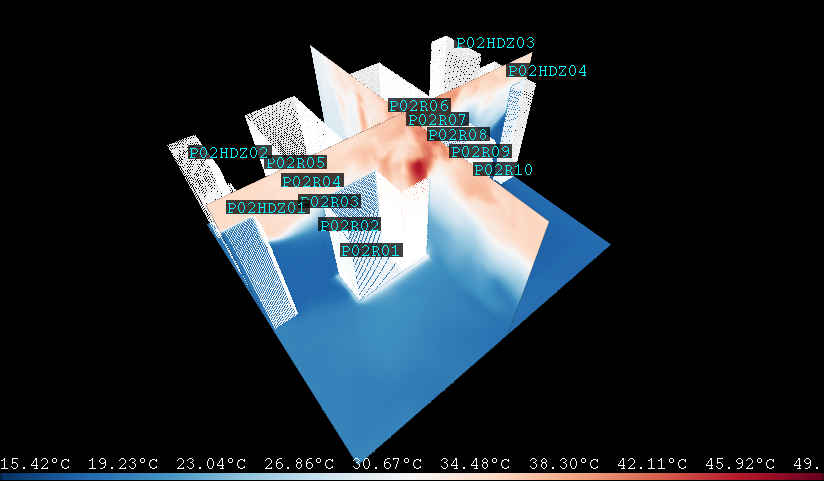
\includegraphics[width=\linewidth]{rafsine_pod2.jpg}
\end{center}
\caption{Simulating the thermal model of data center module POD 2.}
\label{fig:pod2_thermal_flow}
\end{figure}
